% =====================================================================
%  c16 —— 原文印刷页 135–141（PDF 第 136–142 页）
%  含：4.7 Primary Fields（4.7.1、4.7.2）与 4.8 Tensor Product Of Highest
%  Weight Representations 的开头部分；插图 Fig. 19。
% =====================================================================

是模不变的。它们对应着其他的理论。

对 $G=SU(2)$，模不变量具有 ADE 分类，见 Capelli、Itzkyson、Zuber 的一篇漂亮论文。

对 $G=SU(3)$，分类由 Terry Gannon 完成（hep-th/9212060、hep-th/9404185）。论文 hep-th/9604104："Comments on the Links between su(3) Modular Invariants, Simple Factors in the Jacobian of Fermat Curves, and Rational Triangular Billiards"（作者 M. Bauer、A. Coste、C. Itzykson、P. Ruelle）揭示了与数学各个分支之间引人入胜的联系。

对更高秩的群，完整的分类尚属未知（？）

{\small\itshape ［原文标记：数学家对朴素的对角模不变量有些意见。这一点我是从 A. Neitzke 那里得知的。（2019 年 5 月 8 日）］}
% [原文待办标记，原文 p.135；原文以两行星号分隔线上下框住这段全大写文字，所标记的是「朴素的对角模不变量」这一选择在数学上的问题]

\subsection{主场} % 原文: 4.7 Primary Fields

态–算符对应：主场顶点算符

全纯因子化：手征顶点算符。

COMMENT：顶点算符代数（vertex operator algebras）与纯代数进路。（Borcherds、FLM、Lepowsky–Huang 等）

OPE–融合规则：F 矩阵。自洽性：五边形公理。

惊喜！$S$ 对角化融合规则！Verlinde 公式。

\subsubsection{半单代数} % 原文: 4.7.1 Semisimple Algebras

评注：关于一般半单代数的"Verlinde 公式"。给出有限群环的例子。练习：有限群论中的融合规则与 Verlinde 公式。

一般而言，事情就到此为止。不过，当该代数 $(\mathcal{C},\theta)$ 是半单的时候，还可以多说一点。

半单性最为有用的刻画如下。结构常数\footnote{结构常数 $N_{\mu\nu}^{\ \ \lambda}$ 不必是整数。但在许多有趣的例子中，代数存在一组基，使得它们在事实上取整数值。}
\begin{equation}
  \phi_\mu\phi_\nu=N_{\mu\nu}^{\ \ \lambda}\phi_\lambda
  \tag{4.189}
  \label{eq:4.189}
\end{equation}
这些结构常数通过左正则表示（left-regular representation）$L(\phi_\mu)$ 定义出一族矩阵，其矩阵元为 $N_{\mu\nu}^{\ \ \lambda}$。由于 $\mathcal{C}$ 可交换，这些矩阵两两交换。于是：

\textbf{定义}：$\mathcal{C}$ 是半单的，当且仅当矩阵 $L(\phi_\mu)$ 可同时对角化。

于是，在半单情形我们可以找到矩阵 $S$，使得
\begin{equation}
  N_{\mu\nu}^{\ \ \lambda}=\sum_x S_\nu^{\ x}\Lambda_x^{(\mu)}(S^{-1})_x^{\ \lambda}
  \tag{4.190}
  \label{eq:4.190}
\end{equation}

其中 $\Lambda_x^{(\mu)}$ 是 $L(\phi_\mu)$ 的各不相同的本征值。

现在我们选取一组基，使指标 $\mu$ 取遍 $\mu=0,\dots,n$，并取 $\phi_0=1_{\mathcal{C}}$，即乘法单位元。把 $\mu=0$ 代入 \eqref{eq:4.190} 得到的只是一个平凡的恒等式；但若代入 $\nu=0$，并利用 $N_{\mu\nu}^{\ \ \lambda}=N_{\nu\mu}^{\ \ \lambda}$（从而 $N_{\mu 0}^{\ \ \lambda}=\delta_\mu^{\ \ \lambda}$），我们便看出 $S_0^{\ x}\Lambda_x^{(\mu)}=S_\mu^{\ x}$，因为这里用到的正是 $S^{-1}$ 的矩阵逆（即 $S$ 本身）。故
\begin{equation}
  S_0^{\ x}\Lambda_x^{(\mu)}=S_\mu^{\ x}\qquad\qquad\text{no sum on }x
  \tag{4.191}
  \label{eq:4.191}
\end{equation}

把它代回 \eqref{eq:4.190}，我们得到
\begin{equation}
  N_{\mu\nu}^{\ \ \lambda}=\sum_x\frac{S_\nu^{\ x}S_\mu^{\ x}(S^{-1})_x^{\ \lambda}}{S_0^{\ x}}
  \tag{4.192}
  \label{eq:4.192}
\end{equation}
% [Tutor Note: 原稿把矩阵指标排成「错位」形式：$N_{\mu\nu}^{\ \ \lambda}$、$S_\nu^{\ x}$、$(S^{-1})_x^{\ \lambda}$ 里最后一个指标特意错开一格，表示它与 $\mu,\nu$ 不同类（$\mu,\nu$ 是代数乘积的下指标，另一个是基指标）。转写时若丢掉 \ 留出的空位，就会误以为 $x$ 是紧贴 $S_\nu$ 的第一上标，从而把 (4.192) 的分子读错。(4.190) 的矩阵含义是 $L(\phi_\mu)=S\Lambda^{(\mu)}S^{-1}$（矩阵元为 $(L(\phi_\mu))_\nu^{\ \lambda}=N_{\mu\nu}^{\ \ \lambda}$）；核对时把它与 (4.190) 逐项对照，即可确认 $S_\nu^{\ x}$ 与 $(S^{-1})_x^{\ \lambda}$ 的配对，也能看出 (4.191) 为何必须标注「no sum on $x$」：该式对每个 $x$ 单独成立，$x$ 是标记本征值的标号而非求和指标]

注意 $\theta(\phi_\mu\phi_\nu\phi_\lambda)=N_{\mu\nu}^{\ \ \lambda'}Q_{\lambda'\lambda}:=N_{\mu\nu\lambda}$ 关于 $\mu,\nu,\lambda$ 全对称。假设我们进一步把注意力限制在满足 $\theta(\phi_\mu)=\delta_{\mu,0}$ 的基 $\{\phi_\mu\}$ 上。那么对 \eqref{eq:4.189} 取迹便知 $Q_{\mu\nu}=N_{\mu\nu}^{\ \ 0}$，而 \eqref{eq:4.192} 随后给出
\begin{equation}
  Q_{\mu\nu}=\sum_x S_\nu^{\ x}S_\mu^{\ x}\frac{(S^{-1})_x^{\ 0}}{S_0^{\ x}}
  \tag{4.193}
  \label{eq:4.193}
\end{equation}
从而
\begin{equation}
  N_{\mu\nu\lambda}=\sum_x S_\mu^{\ x}S_\nu^{\ x}S_\lambda^{\ x}\frac{(S^{-1})_x^{\ 0}}{(S_0^{\ x})^2}
  \tag{4.194}
  \label{eq:4.194}
\end{equation}

若作线性组合
\begin{equation}
  \epsilon_x=\sum_\mu S_0^{\ x}(S^{-1})_x^{\ \mu}\phi_\mu
  \tag{4.195}
  \label{eq:4.195}
\end{equation}
则 $\epsilon_x$ 构成一组基本幂等元（basic idempotents），即
\begin{equation}
  \begin{gathered}
    \mathcal{C}=\oplus_x\mathbb{C}\epsilon_x\\
    \epsilon_x\epsilon_y=\delta_{x,y}\epsilon_y
  \end{gathered}
  \tag{4.196}
  \label{eq:4.196}
\end{equation}
% [Tutor Note: 「$\epsilon_x$ 给出 $\mathcal{C}$ 的直和分解」等价于有限维可交换半单代数（且带非退化对称双线性型，即本文的 $\theta$）的结构定理——Artin–Wedderburn 定理的交换情形，作者此处写 "that is" 直接给出，未作证明。被略去的一步是：$L(\phi_\mu)$ 可同时对角化 $\Rightarrow$ 存在公共本征向量基 $\Rightarrow$ Lagrange 插值可构造出两两正交的幂等元；反过来由幂等元存在则 $L(\phi_\mu)$ 在基 $\epsilon_x$ 下对角。这一步与 $\theta$ 无关，纯属线性代数，可查任意一本代数教材的「半单代数」一节]

此外，若取自然归一化 $\theta(\phi_\mu)=\delta_{\mu,0}$，则
\begin{equation}
  \theta_x:=\theta_{\mathcal{C}}(\epsilon_x)=S_0^{\ x}(S^{-1})_x^{\ 0}
  \tag{4.197}
  \label{eq:4.197}
\end{equation}

这里 $\theta_i$ 是一些非零复数。无序集合 $\{\theta_x\}$ 是有限维可交换半单 Frobenius 代数的唯一不变量。
% [Tutor Note: 原文此处写 $\theta_i$，而前后文一律用 $\{\theta_x\}$（$x$ 标记幂等元、$\mu,\nu,\lambda$ 标记基元素），从 (4.197) 的指标也可看出应为 $\theta_x$。译文照原文转写 $\theta_i$ 未改，但引用 (4.197)、(4.199)、(4.200) 时应按 $\theta_x$ 理解]

% [原文标记：此处有两行纯星号分隔线（原稿的分段记号，无文字），原文 p.136]
{\small\itshape ［原文标记：以下部分材料应当移到"拓扑场论"一章——二维 TFT 的例子：］}
% [原文待办标记，原文 p.136；作者希望把随后关于二维 TFT 的整段讨论挪到拓扑场论一章]

注意在此情形，特征元（characteristic element）简单地就是
\begin{equation}
  H=\sum_x\frac{1}{\theta_x}\epsilon_x
  \tag{4.198}
  \label{eq:4.198}
\end{equation}
从而在亏格为 $g\ge0$ 的曲面上的真空振幅为
\begin{equation}
  Z_g=\sum_x\theta_x^{1-g}
  \tag{4.199}
  \label{eq:4.199}
\end{equation}

\textbf{评注}：

\begin{enumerate}
  \item 若考虑对所有亏格的求和，则该求和只在 $|\theta_x|>1$ 时收敛（在单位圆上为条件收敛），此时它等于
  \begin{equation}
    Z_{\mathrm{string}}=\sum_x\frac{\theta_x}{1-\theta_x^{-1}}
    \tag{4.200}
    \label{eq:4.200}
  \end{equation}

  \item 注意至此还没有任何东西固定矩阵 $S$ 的整体归一化。在某些情形 $S$ 是幺正的，从而 $(S^{-1})_x^{\ 0}=(S_0^{\ x})^*$。此外，若矩阵元 $S_0^{\ x}$ 可以取为实数，则 \eqref{eq:4.194} 有一个漂亮的简化：
  \begin{equation}
    N_{\mu\nu\lambda}=\sum_x\frac{S_\mu^{\ x}S_\nu^{\ x}S_\lambda^{\ x}}{S_0^{\ x}}
    \tag{4.201}
    \label{eq:4.201}
  \end{equation}
\end{enumerate}

这正是 Verlinde 公式通常的表述形式。

\textbf{练习}\quad 证明本征值 $\Lambda_x^{(\rho)}$ 满足代数关系
\begin{equation}
  \Lambda_x^{(\mu)}\Lambda_x^{(\nu)}=\sum_\lambda N_{\mu\nu}^{\ \ \lambda}\Lambda_x^{(\lambda)}
  \tag{4.202}
  \label{eq:4.202}
\end{equation}

\textbf{练习}\quad 场论中一个自然的问题是：一个理论的真空振幅是否完全决定了该理论中的一切振幅。请就半单二维 TFT 的情形研究这一问题。

% [原文标记：此处有两行纯星号分隔线（原稿的分段记号，无文字），原文 p.137]

\subsubsection{半单融合规则的一个例子：有限群论} % 原文: 4.7.2 An Example Of Semisimple Fusion Rules: Finite Group Theory

设 $G$ 为有限群。复值函数空间 $\mathbb{C}[G]$ 在逐点乘法给出的显然乘积
\begin{equation}
  f_1\cdot f_2(g):=f_1(g)f_2(g)
  \tag{4.203}
  \label{eq:4.203}
\end{equation}
之下是一个 $C^*$ 代数（见下文）。

令 $\mathcal{C}$ 为类函数（class functions）的子空间，即满足
\begin{equation}
  f(hgh^{-1})=f(g)\qquad\forall g,h\in G
  \tag{4.204}
  \label{eq:4.204}
\end{equation}
的函数全体。这是 $G$ 的（有限个）共轭类所成集合上的函数空间。

$\mathcal{C}$ 有两组自然的函数基。其中一组使 $\mathcal{C}$ 显然以自然的方式成为一个 Frobenius 代数，另一组则使这个 Frobenius 代数的半单性一目了然。

类函数空间的第一组自然基由各不相同的不可约表示的特征标 $\chi_\mu$ 给出，$\mu$ 标记 $G$ 的各不相同的不可约表示。

在逐点乘法下
\begin{equation}
  \chi_\mu\chi_\nu=\sum_\lambda N_{\mu\nu}^{\ \ \lambda}\chi_\lambda
  \tag{4.205}
  \label{eq:4.205}
\end{equation}
其中 $N_{\mu\nu}^{\ \ \lambda}$ 是融合系数（fusion coefficients）（它们也被称为"Littlewood–Richardson 系数"）。它们由 Clebsch–Gordon 级数
\begin{equation}
  T^\mu\otimes T^\nu=\oplus_\lambda N_{\mu\nu}^{\ \ \lambda}T^\lambda
  \tag{4.206}
  \label{eq:4.206}
\end{equation}
确定，并且是非负整数。自然的迹为
\begin{equation}
  \theta(\chi_\mu)=\delta_{\mu,0}
  \tag{4.207}
  \label{eq:4.207}
\end{equation}
其中 $\chi_0=1$ 对应平凡表示。由于对每个表示 $\mu$ 都存在表示 $\mu^*$ 使得 $\chi_\mu\chi_{\mu^*}=\chi_0+\cdots$，我们断定 $\langle f,g\rangle=\theta(fg)$ 非退化，从而 $\mathcal{C}$ 确实是一个 Frobenius 代数。

类函数的另一组自然基是共轭类上的 delta 函数：
\begin{equation}
  \begin{aligned}
    \delta_C(g)&=1&&g\in C\\
    &=0&&g\notin C
  \end{aligned}
  \tag{4.208}
  \label{eq:4.208}
\end{equation}
其中 $C$ 是一个共轭类。注意在这组基下，逐点乘法是对角的。于是 $\mathcal{C}$ 的半单性便是显然的。

我们当然可以把一组基按另一组展开：
\begin{equation}
  \chi_\mu=\sum_i\chi_\mu(C_i)\delta_{C_i}
  \tag{4.209}
  \label{eq:4.209}
\end{equation}

现在回忆群表示论中的一个标准结果：不可约表示的特征标所满足的正交关系
\begin{equation}
  \frac{1}{|G|}\sum_g\chi_\mu(g)\chi_\nu(g^{-1})=\delta_{\mu,\nu}
  \tag{4.210}
  \label{eq:4.210}
\end{equation}

由于 $G$ 有限，不失一般性（WLOG）可假定表示 $T^\mu$ 是幺正的。因此矩阵
\begin{equation}
  S_{i\mu}=\sqrt{\frac{m_i}{|G|}}\chi_\mu(C_i)
  \tag{4.211}
  \label{eq:4.211}
\end{equation}
（其中 $m_i$ 是类 $|C_i|$ 的阶）是幺正矩阵。

现在我们有
\begin{equation}
  \chi_\mu=\sum_i\sqrt{\frac{|G|}{m_i}}S_{i\mu}\delta_{C_i}
  \tag{4.212}
  \label{eq:4.212}
\end{equation}
因此，由于乘法在基 $\delta_{C_i}$ 下是对角的，$S_{i\mu}$ 就是在特征标基下对角化融合规则的那个矩阵。
% [Tutor Note: (4.211) 的幺正性来自 (4.210)：把 $\sum_g$ 按共轭类分组后，$\sum_g\chi_\mu(g)\chi_\nu(g^{-1})=\sum_i m_i\chi_\mu(C_i)\chi_\nu(C_i)$（用了 $\chi_\nu(g^{-1})=\chi_\nu(g)^*$，这正是「$T^\mu$ 可取幺正」的作用），代入 (4.211) 即得 $\sum_i S_{i\mu}S_{i\nu}^*=\delta_{\mu\nu}$。另需注意原文 "where $m_i$ is the order of the class $|C_i|$" 的措辞含糊：$m_i$ 就是共轭类 $C_i$ 的元素个数，即 $m_i=|C_i|$，与记号 $|C_i|$ 指同一个量，(4.214) 中的 $|G|$ 则是群的阶，勿混]

现在，利用 \eqref{eq:4.197} 我们算得
\begin{equation}
  \theta_x=|S_{0x}|^2=\frac{(\dim V_x)^2}{|G|}
  \tag{4.213}
  \label{eq:4.213}
\end{equation}

{\small\itshape ［原文标记：把这一段移到"拓扑场论——二维例子"一章。］}
% [原文待办标记，原文 p.139；该行上、下各有一行星号分隔线]

从而亏格为 $g$ 的紧 Riemann 面上的配分函数为
\begin{equation}
  Z_g=|G|^{1-g}\sum_x\frac{1}{(\dim V_x)^{2g-2}}
  \tag{4.214}
  \label{eq:4.214}
\end{equation}
其中求和遍历 $G$ 的全部不可约表示。第一个因子相对无趣（它可以被吸收进弦耦合常数的标度之中），但第二个因子很有趣。

\emph{\eqref{eq:4.214} 中的求和究竟在计数什么样的几何对象？}

我们将在随后几讲中回答这个问题。

% [原文标记：此处有两行纯星号分隔线（原稿的分段记号，无文字），原文 p.140]

\textbf{练习}
\begin{enumerate}[label=\alph*.)]
  \item 证明带卷积乘积的群代数 $\mathbb{C}[G]$ 的中心就是 $\mathcal{C}$，即类函数空间。
  \item 证明矩阵 $S_{i\mu}$ 是 $\mathcal{C}$ 上这两种乘积结构之间的一种 Fourier 变换。注意各不可约表示的特征标基 $\chi_\mu$ 对角化卷积乘积：
  \begin{equation}
    \chi_\mu*\chi_\nu=\frac{\delta_{\mu\nu}}{n_\nu}\chi_\nu
    \tag{4.215}
    \label{eq:4.215}
  \end{equation}
  \item 证明这个 Frobenius 代数的诸不变量 $\theta_x$ 由
  \begin{equation}
    \theta(\epsilon_\mu)=\frac{(\dim V_\mu)^2}{|G|}
    \tag{4.216}
    \label{eq:4.216}
  \end{equation}
  给出。
\end{enumerate}
% [Tutor Note: 原文用斜体 $C[G]$ 表示复群代数（即 $\mathbb{C}[G]$），与类函数子空间的花体 $\mathcal{C}$ 只是同一字母的两种字体，含义完全不同；译文以 $\mathbb{C}[G]$ 与 $\mathcal{C}$ 区分，避免混淆。又，原文本节把 $S_{i\mu}$ 的下标排成「类在前、不可约表示在后」，而 (4.197) 中的 $S$ 是「指标 $x$ 在前」；两处 $S$ 相差转置与相位约定（(4.213) 只用到 $|S_{0x}|^2$，故不受影响），逐式核对时需留意]

\begin{figure}[htbp]
  \centering
  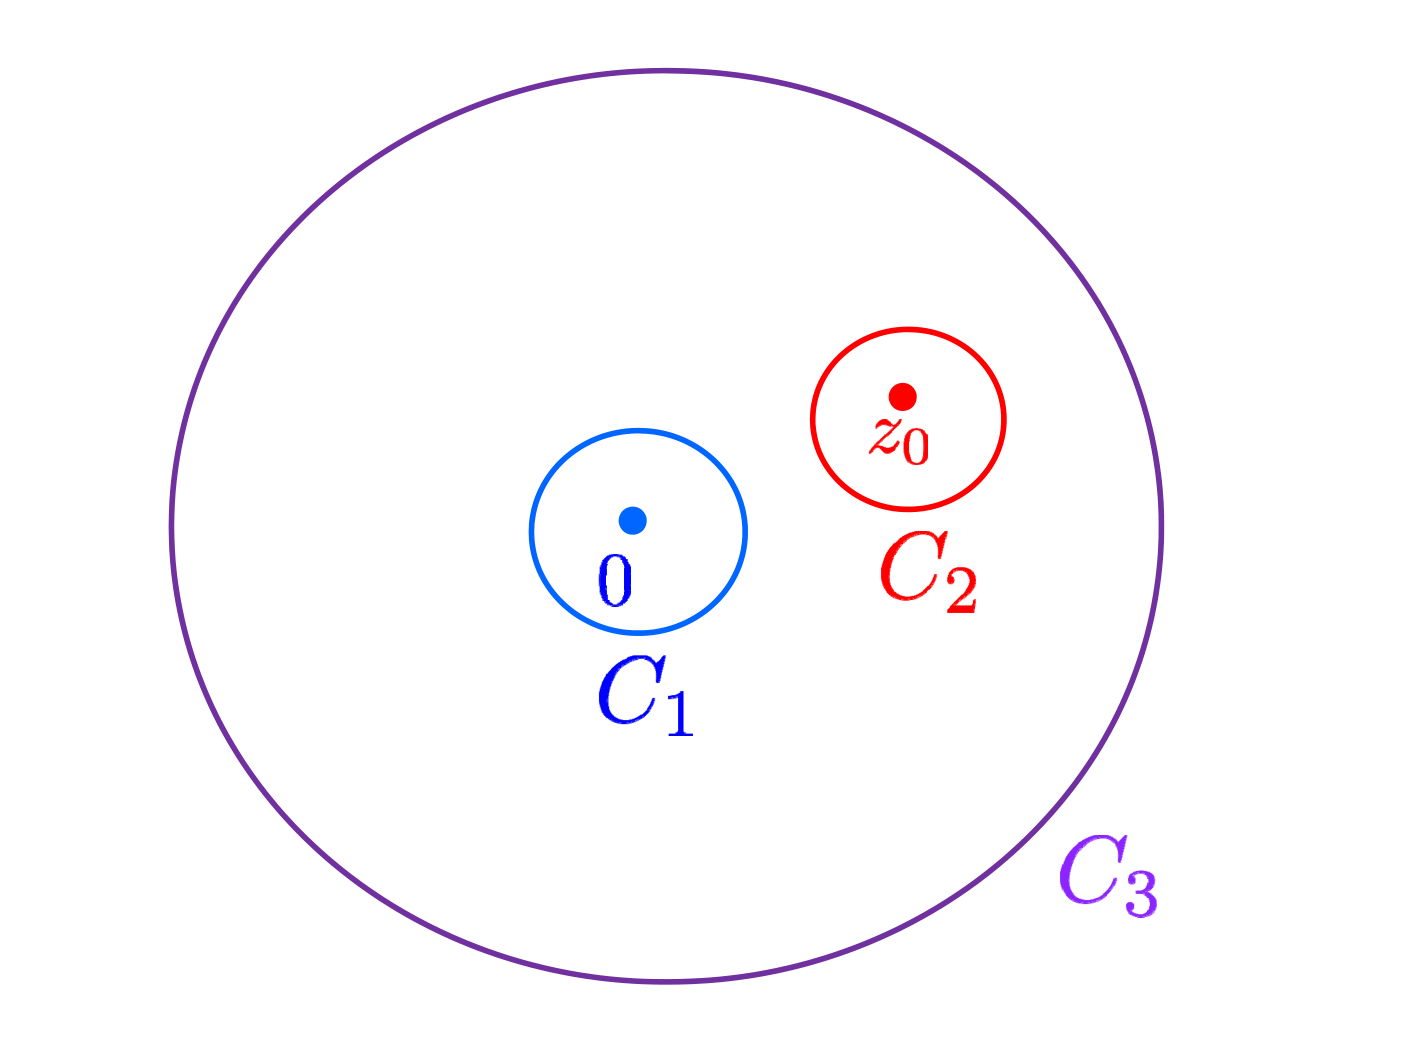
\includegraphics[width=0.55\textwidth]{figures/fig19.png}
  \caption{三个 CFT 状态空间分别与圆 $C_1$、$C_2$、$C_3$ 相关联，它们分别对应于围绕 $z=0$、$z_0$、$0$ 的径向量子化。（原文 Fig.~19，第 140 页）}
  \label{fig:19}
\end{figure}

\subsection{最高权表示的张量积} % 原文: 4.8 Tensor Product Of Highest Weight Representations

可积最高权表示 $L(\lambda)$ 原来是张量范畴（tensor category）中的对象。张量积并不是对称的。注意，要取两个表示 $L(\lambda)$ 与 $L(\lambda')$ 的张量积、以得到同一个 $k$ 值的 KM 代数的表示，这并非显然。\footnote{出于同样的理由，人们也不愿意把特征标相乘。} 做到这一点的办法是利用共形场论。

张量积可以这样理解。（我们沿用 [42] 式 (2.5) 的描述。利用顶点算符代数理论对张量积的严格描述见 [29, 30]。）

我们可以构造一个流：
\begin{equation}
  J^a(z)=\sum T_n^a z^{-n-1}dz
  \tag{4.217}
  \label{eq:4.217}
\end{equation}
其中我们现在把 $z$ 解析延拓到复平面——把它看作 WZW 模型的二维欧氏 QFT 的欧氏世界面。注意
\begin{equation}
  T_n^a=\oint z^nJ^a(z)
  \tag{4.218}
  \label{eq:4.218}
\end{equation}

存在态–算符对应：在平面上的点 $z$ 处插入一个局部算符 $\Phi(z)$，会在以该点为中心的径向量子化的 Hilbert 空间中产生一个态。

要给出张量积，我们需要一个余乘法（comultiplication）$\Delta:\mathcal{A}\to\mathcal{A}\otimes\mathcal{A}$，其中 $\mathcal{A}$ 是局部可观测量的代数。

设想：在以 $z=0$ 为中心的小圆 $C_1$ 上有第一个态的 Hilbert 空间，在以 $z=z_0$ 为中心的第二个圆 $C_2$ 上有第二个，而在以 $z=0$ 为中心、但环绕 $z_0$ 的第三个更大的圆 $C_3$ 上有第三个。见图~\ref{fig:19}。

若在 $z=0$ 与 $z=z_0$ 处插入在表示 $L_\lambda$ 与 $L_\mu$ 中产生态的局部算符，则圆 $C_3$ 上所得到的态将带有流的作用，其模为
\begin{equation}
  \begin{aligned}
    \Delta_{0,z_0}(T_n^a)&=\oint_{C_3}z^nJ^a(z)\\
    &=\left(\oint_{C_1}z^nJ^a(z)\right)\otimes 1+1\otimes\left(\oint_{C_2}z^nJ^a(z)\right)
  \end{aligned}
  \tag{4.219}
  \label{eq:4.219}
\end{equation}
第一行写的是作用在圆 $C_3$ 上态空间的一个算符。（可以把它想成一条裤子图（pair of pants）中的出射态空间。）下一行是一次围道形变（因为 $J^a(z)$ 是全纯流），以给出对圆 $C_1$ 与 $C_2$ 上态空间的作用。由于裤子图上有两个入射态，我们得到的是态空间的张量积。有趣的一项是 $\oint_{C_2}z^nJ^a(z)\,dz$。当作用在以 $z_0$ 为中心的径向量子化所得的 Hilbert 空间上时，我们应把流展开为
\begin{equation}
  J^a(z)=\sum_{m\in\mathbb{Z}}(z-z_0)^{-m-1}J_m^a(z_0)\,d(z-z_0)
  \tag{4.220}
  \label{eq:4.220}
\end{equation}
但
\begin{equation}
  \oint_{C_2}z^n(z-z_0)^{-m-1}dz=
  \begin{cases}
    0 & m\le-1\\
    \binom{n}{m}z_0^{n-m} & m\ge0
  \end{cases}
  \tag{4.221}
  \label{eq:4.221}
\end{equation}
从而
\begin{equation}
  \Delta_{0,z_0}(T_n^a)=T_n^a\otimes 1+1\otimes\left(\sum_{k=0}^{\infty}\binom{n}{k}z_0^{n-k}T_k^a(z_0)\right)
  \tag{4.222}
  \label{eq:4.222}
\end{equation}
% [Tutor Note: (4.221) 的二项式系数来自留数而非展开系数的直接读取：(4.220) 的展开点是 $z_0$，而围道积分号里带的是 $z^n=((z-z_0)+z_0)^n$，其 $z_0^{n-m}(z-z_0)^m$ 项与 $(z-z_0)^{-m-1}$ 相乘后给出 $(z-z_0)^{-1}$ 的留数，故系数为 $\binom{n}{m}z_0^{n-m}$；同时 (4.220) 的微分是 $d(z-z_0)$ 而文中被积式写的是 $dz$，两者相等，但若误把 (4.220) 的 $dz$ 漏掉就会丢掉 $(z-z_0)^{-m-1}$ 这一幂次的来源。此外 (4.222) 中的 $T_k^a(z_0)$ 带上了展开点 $z_0$，与 (4.217) 中无自变量的 $T_n^a$ 不是同一个记号，对照时勿混]

现在，简单对象（即 $G_k$ 的不可约表示）在这一张量积下的乘法融合规则，原来定义出一个半单 Frobenius 代数：\footnote{其概念上的理由是：可以把 WZW 模型的 $G$ 对称性规范化，从而得到 $G/G$ 模型。这是一个二维 TFT。}
\begin{equation}
  L(\mu)\otimes_{0,z_0}L(\nu)\cong\oplus_\lambda N_{\mu\nu}^{\ \ \lambda}L(\lambda).
  \tag{4.223}
  \label{eq:4.223}
\end{equation}

因此，存在一个矩阵 $S$ 对角化这些规则。
% [Tutor Note: 原文用 "turn out to define" 一笔带过 (4.223) 中「半单性 + Frobenius 结构」的验证，被省略的实质内容是：$G_k$（能级 $k$ 的仿射 KM 代数）的可积表示在共形场论给出的张量积下融合系数非负、结合（由共形块的结合律 / 五边形方程保证），且存在非退化不变配对使融合代数成为半单 Frobenius 代数——这正是 Verlinde 公式成立的前提。作者在脚注中提示的 $G/G$ 模型给出的是一条概念性论证思路；严格证明可查 [42] 所引的文献，以及本章前文关于 $S$ 矩阵与融合规则关系的讨论]
